% -------------------------------------------------------------------------
%  fig-scaling.tex  --  measured thread scaling
%
%  MONOCHROME: every \addplot carries an explicit black stroke and is
%  distinguished by mark shape plus dash pattern.  Do NOT use \addplot+ here --
%  the "+" appends pgfplots' default cycle list, which is coloured.
% -------------------------------------------------------------------------
\newcommand{\FigScaling}{%
\begin{figure}[tb]
\centering
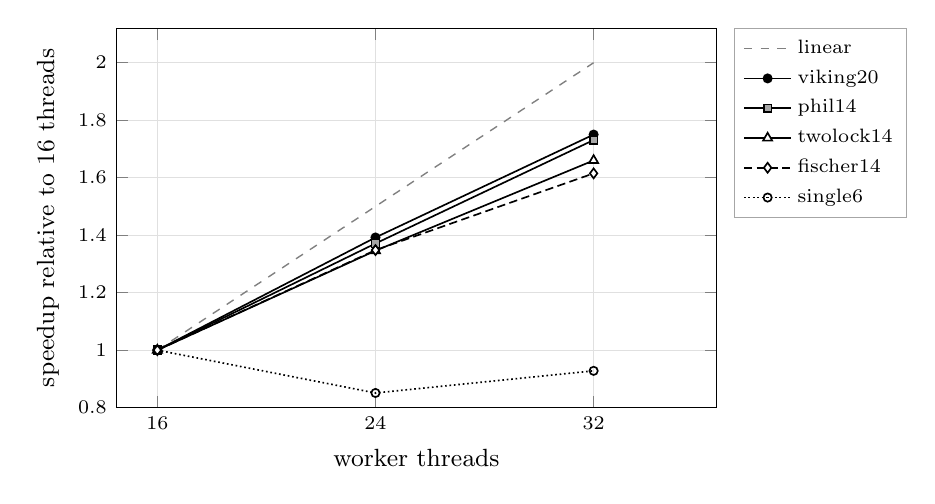
\begin{tikzpicture}
\begin{axis}[
  width=92mm, height=64mm,
  xlabel={worker threads},
  ylabel={speedup relative to $16$ threads},
  xtick={16,24,32}, xmin=14.5, xmax=36.5, ymin=0.8, ymax=2.12,
  ytick={0.8,1.0,1.2,1.4,1.6,1.8,2.0},
  grid=major, grid style={black!12, line width=0.3pt},
  tick label style={font=\scriptsize},
  label style={font=\small},
  legend style={font=\scriptsize, draw=black!35, fill=white,
                at={(1.03,1.0)}, anchor=north west, cells={anchor=west},
                row sep=0.4pt},
  legend cell align=left,
]
\addplot[black!50, dashed, line width=0.5pt, mark=none]
  coordinates {(16,1.0) (24,1.5) (32,2.0)};       \addlegendentry{linear}
\addplot[black, line width=0.6pt, mark=*, mark size=1.5pt,
         mark options={fill=black}]
  coordinates {(16,1.000) (24,1.392) (32,1.750)}; \addlegendentry{viking20}
\addplot[black, line width=0.6pt, mark=square*, mark size=1.4pt,
         mark options={fill=black!35}]
  coordinates {(16,1.000) (24,1.371) (32,1.731)}; \addlegendentry{phil14}
\addplot[black, line width=0.6pt, mark=triangle*, mark size=1.9pt,
         mark options={fill=white}]
  coordinates {(16,1.000) (24,1.346) (32,1.660)}; \addlegendentry{twolock14}
\addplot[black, line width=0.6pt, dash pattern=on 3pt off 1.6pt,
         mark=diamond*, mark size=1.8pt, mark options={solid, fill=white}]
  coordinates {(16,1.000) (24,1.348) (32,1.615)}; \addlegendentry{fischer14}
\addplot[black, line width=0.6pt, densely dotted, mark=o, mark size=1.5pt,
         mark options={solid}]
  coordinates {(16,1.000) (24,0.851) (32,0.928)}; \addlegendentry{single6}
\end{axis}
\end{tikzpicture}
\caption{Measured scaling from $16$ to $32$ workers on the large instances of
each family (wall-clock, best of two runs, \code{--omp-chunk 8}).  Doubling the
worker count buys $1.62$--$1.75\times$, i.e.\ $81$--$87\%$ parallel efficiency
in that range, on every family whose state space is spread over many discrete
states.  \code{single6} is the deliberate counterexample: it is a single
automaton with one location and $N$ independent clocks, so its \emph{entire}
passed set is one discrete state -- one stripe, one antichain, one lock -- and
no amount of hardware helps.  That is a property of the model, not of the
implementation, and it is the honest boundary of this design.}
\label{fig:scaling}
\end{figure}}
